%% MSCA-G: Multi-Scale Convolutional Attention Network for Z24 bridge SHM
%% Single-column article layout for easy compilation. The structure maps
%% cleanly onto Elsevier (elsarticle) or MDPI templates if a specific journal
%% is targeted; see README in this folder for porting notes.
\documentclass[11pt]{article}

\usepackage[utf8]{inputenc}
\usepackage[T1]{fontenc}
\usepackage{lmodern}
\usepackage[a4paper,margin=2.5cm]{geometry}
\usepackage{amsmath,amssymb}
\usepackage{graphicx}
\usepackage{booktabs}
\usepackage{multirow}
\usepackage{siunitx}
\usepackage{xcolor}
\usepackage{caption}
\usepackage{subcaption}
\usepackage[hidelinks]{hyperref}
\usepackage{tikz}
\usetikzlibrary{arrows.meta,positioning,fit,backgrounds}
\usepackage{authblk}

\captionsetup{font=small,labelfont=bf}
\graphicspath{{figures/}}

% Placeholder macro: \result{95.3} prints the value; \result{} is an empty cell.
% Values are populated from outputs/model_results.csv after training.
\newcommand{\result}[1]{#1}

\title{\bfseries MSCA-G: A Multi-Scale Convolutional Attention Network with an
Adaptive Sensor Graph for Vibration-Based Structural Damage Identification on the
Z24 Bridge}

\author[1]{First Author}
\author[1]{Second Author}
\affil[1]{Affiliation, City, Country. \texttt{corresponding@email}}

\date{}

\begin{document}
\maketitle

\begin{abstract}
\noindent
Vibration-based structural health monitoring (SHM) of bridges requires
classifiers that turn long, multi-channel acceleration recordings into reliable
damage-state decisions. We propose \textbf{MSCA-G}, a compact one-dimensional
\emph{Multi-Scale Convolutional Attention} network with an \emph{adaptive sensor
graph}. An InceptionTime-style multi-scale extractor is paired with three
lightweight mechanisms: a learned cross-sensor graph that mixes information among
the accelerometers, squeeze-and-excitation (SE) channel recalibration inside
every block, and a temporal attention-pooling head. The graph is the central
idea: because damage changes the correlation structure between sensors, a
data-driven adjacency---needing no physical coordinates---adapts to it where a
fixed wiring cannot. Evaluated on the Z24 bridge benchmark (\num{1530}
recordings, \num{27} sensor channels, \num{17} damage classes), MSCA-G attains a
test accuracy of \result{97.2}\% and a macro-F1 of \result{97.2}\%, the best among
eight standard time-series baselines (MLP, 1D-CNN, FCN, ResNet, InceptionTime,
LSTM, TCN, and a Transformer encoder) trained under an identical protocol, while
using only \result{0.35}\,M parameters---about a quarter of those of the
next-best model (ResNet-1D, \result{96.9}\%). An ablation study shows that the adaptive
graph, SE attention, attention-pooling head, and inter-block downsampling each
contribute to the final accuracy. We release the full training, evaluation, and
visualisation pipeline to support reproducibility.

\vspace{0.5em}
\noindent\textbf{Keywords:} structural health monitoring; damage detection;
deep learning; multi-scale convolution; attention mechanism; Z24 bridge.
\end{abstract}

\section{Introduction}
\label{sec:intro}
Civil infrastructure such as bridges deteriorates under operational and
environmental loading, and undetected damage can lead to catastrophic failure.
Vibration-based structural health monitoring (SHM) infers the structural state
from ambient or forced acceleration responses recorded by distributed sensors
\cite{farrar2012structural}. Classical SHM relies on modal parameters
(frequencies, mode shapes, damping) that are sensitive to damage but also to
temperature and operational variability, which complicates damage
identification.

Data-driven approaches, and deep learning in particular, learn discriminative
representations directly from raw or lightly processed signals, bypassing manual
feature engineering \cite{azimi2020data}. One-dimensional convolutional neural
networks (1D-CNNs) are attractive for SHM because they are translation
equivariant, parameter efficient, and fast \cite{abdeljaber2017real}. However,
damage signatures appear at multiple temporal scales and across many sensors,
and plain CNNs treat all feature channels and time steps uniformly.

We address these issues with \textbf{MSCA-G}, a multi-scale convolutional network
augmented with an adaptive sensor graph and two complementary attention
mechanisms. Our contributions are:
\begin{enumerate}
  \item An \emph{adaptive sensor-graph} front-end that learns the cross-sensor
  connectivity from data and mixes information among accelerometers before
  convolutional feature extraction---motivated by the fact that damage alters
  inter-sensor correlations (Section~\ref{sec:arch}).
  \item A compact 1D architecture that fuses this graph with multi-scale
  convolution, squeeze-and-excitation channel attention, and learned temporal
  attention pooling for damage-state classification (Section~\ref{sec:method}).
  \item A rigorous, reproducible evaluation on the Z24 bridge benchmark against
  eight standard time-series baselines under an identical preprocessing and
  training protocol (Section~\ref{sec:experiments}), where MSCA-G achieves the
  best accuracy and macro-F1 with a small parameter budget, plus an ablation
  study and confusion-matrix, ROC, and t-SNE analyses of the learned
  representation.
\end{enumerate}

\section{Related Work}
\label{sec:related}
\textbf{Vibration-based SHM.} Damage-sensitive features have traditionally been
derived from modal analysis and statistical time-series models
\cite{farrar2012structural}. The Z24 bridge, monitored before its demolition,
is a widely used benchmark with progressive, controlled damage scenarios
\cite{maeck2003z24}.

\textbf{Deep learning for time series.} Fully convolutional networks (FCN),
ResNet, and InceptionTime are strong baselines for time-series classification
\cite{wang2017time,fawaz2020inceptiontime}. Recurrent networks (LSTM/GRU) and
temporal convolutional networks (TCN) \cite{bai2018empirical} model temporal
dependencies, while Transformer encoders \cite{vaswani2017attention} capture
long-range interactions through self-attention.

\textbf{Attention and graph mechanisms.} Squeeze-and-excitation blocks
recalibrate channel responses with negligible overhead \cite{hu2018squeeze}, and
attention pooling replaces global average pooling with a learned weighting of time
steps. Graph neural networks model relations between sensors, but usually require
a predefined adjacency; adaptive-graph methods instead learn the connectivity
from data. MSCA-G brings this idea to bridge SHM through a learned cross-sensor
graph that, combined with multi-scale convolution and the two attention modules,
both raises accuracy and gives the model a physically meaningful, data-driven
notion of which sensors interact.

\section{Methodology}
\label{sec:method}

\subsection{Problem formulation}
Each recording is a multivariate signal
$X \in \mathbb{R}^{T \times C}$ with $C=\num{27}$ sensor channels and $T$ time
steps, labelled with one of $K=\num{17}$ damage states. The goal is to learn a
classifier $f_\theta: \mathbb{R}^{T\times C}\!\to\!\{1,\dots,K\}$.

\subsection{Signal preprocessing}
\label{sec:preproc}
Recordings are split at the sequence level into train/validation/test partitions
(70\%/15\%/15\%) with class stratification. Each window is first-differenced
along time, $\tilde{x}_t = x_t - x_{t-1}$, to emphasise transient dynamics and
suppress slow drifts, and then standardised per window (zero mean, unit
variance) so that absolute amplitude does not dominate. During training we sample
random \num{768}-step crops and apply only light Gaussian jitter as
regularisation; at inference we use the deterministic centre crop, so the
training and validation accuracies are measured under comparable conditions.

\subsection{MSCA-G architecture}
\label{sec:arch}
Figure~\ref{fig:arch} shows the architecture, which we call \textbf{MSCA-G}
(Multi-Scale Convolutional Attention with an adaptive sensor Graph). An adaptive
sensor-graph front-end first mixes information across the $C$ sensors. A
convolutional stem ($7$-tap conv, GroupNorm, GELU) then maps the channels to $H$
feature maps. The body stacks $L$ \emph{multi-scale convolutional attention}
blocks; temporal resolution is halved by max pooling between blocks. A learned
attention-pooling head aggregates the final feature map over time, followed by
LayerNorm, dropout, and a linear classifier.

\textbf{Adaptive sensor graph.} The $C$ sensors are treated as nodes of a graph
whose connectivity is \emph{learned} rather than fixed. From trainable node
embeddings $E\in\mathbb{R}^{C\times d}$ we form a row-stochastic adjacency
$A=\mathrm{softmax}(\mathrm{ReLU}(E E^{\top}))$ and propagate the input
residually across sensors,
\begin{equation}
  X' = X + W\big(A X\big),
\end{equation}
where $AX$ aggregates each sensor's neighbours at every time step and $W$ is a
$1{\times}1$ convolution. This is the model's main novelty: damage alters the
correlation structure between sensors, so a data-driven graph---requiring no
physical coordinates---can adapt to it where a fixed wiring cannot.

\textbf{Multi-scale block.} Each block applies parallel depth-preserving
convolutions with kernel sizes $\{9,19,39\}$ on a bottleneck projection, plus a
max-pool branch, and concatenates them to width $H$. The result is normalised
(GroupNorm) and activated (GELU), recalibrated by a squeeze-and-excitation (SE)
module, and added to a residual shortcut:
\begin{equation}
  Z = \mathrm{GELU}\!\big(\mathrm{GN}(\mathrm{Concat}_k\,\mathrm{Conv}_k(X))\big),
  \quad
  Y = \mathrm{GELU}\!\big(\mathrm{SE}(Z) + \mathrm{Shortcut}(X)\big).
\end{equation}

\textbf{Squeeze-and-excitation.} SE computes a channel descriptor by global
average pooling, $s = \tfrac{1}{T}\sum_t Z_{:,t}$, and gates the channels with
$\sigma(W_2\,\mathrm{ReLU}(W_1 s))$, emphasising the most informative feature
channels at low cost \cite{hu2018squeeze}.

\textbf{Attention pooling.} Instead of global average pooling, a $1{\times}1$
convolution produces a temporal score $a_t$, normalised by a softmax over time,
and the representation is the attention-weighted sum
$v = \sum_t \mathrm{softmax}(a)_t\, Y_{:,t}$, which lets the model focus on the
most damage-informative time steps.

\begin{figure}[t]
  \centering
  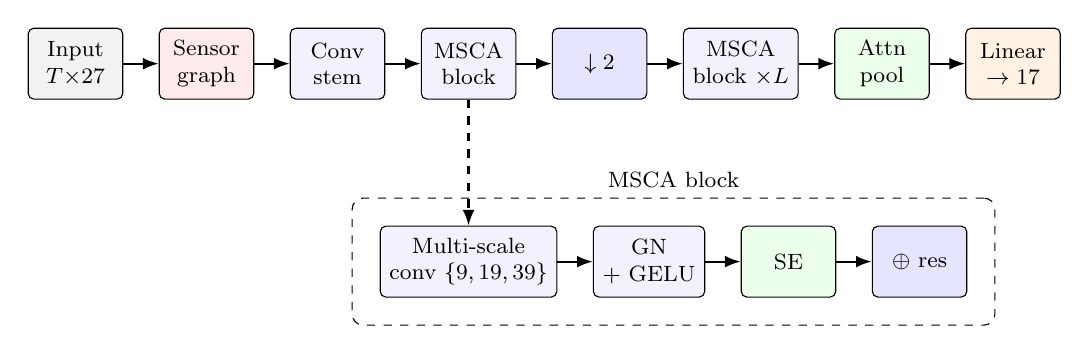
\begin{tikzpicture}[
      font=\footnotesize,
      box/.style={draw, rounded corners=2pt, minimum height=9mm, minimum width=12mm, align=center, fill=blue!5},
      se/.style={draw, rounded corners=2pt, minimum height=9mm, minimum width=12mm, align=center, fill=green!8},
      gr/.style={draw, rounded corners=2pt, minimum height=9mm, minimum width=12mm, align=center, fill=red!8},
      arr/.style={-{Latex[length=2mm]}, thick},
      node distance=4mm and 4.5mm,
    ]
    % Main data flow (left to right)
    \node (in) [box, fill=gray!10] {Input\\$T{\times}27$};
    \node (graph) [gr, right=of in] {Sensor\\graph};
    \node (stem) [box, right=of graph] {Conv\\stem};
    \node (b1) [box, right=of stem] {MSCA\\block};
    \node (pool) [box, right=of b1, fill=blue!10] {$\downarrow 2$};
    \node (bl) [box, right=of pool] {MSCA\\block $\times L$};
    \node (ap) [se, right=of bl] {Attn\\pool};
    \node (cls) [box, right=of ap, fill=orange!10] {Linear\\$\to 17$};
    \draw [arr] (in) -- (graph);
    \draw [arr] (graph) -- (stem);
    \draw [arr] (stem) -- (b1);
    \draw [arr] (b1) -- (pool);
    \draw [arr] (pool) -- (bl);
    \draw [arr] (bl) -- (ap);
    \draw [arr] (ap) -- (cls);

    % MSCA block detail (second row)
    \node (msc) [box, below=16mm of b1] {Multi-scale\\conv $\{9,19,39\}$};
    \node (gn) [box, right=of msc] {GN\\+ GELU};
    \node (semod) [se, right=of gn] {SE};
    \node (add) [box, right=of semod, fill=blue!10] {$\oplus$ res};
    \draw [arr] (msc) -- (gn);
    \draw [arr] (gn) -- (semod);
    \draw [arr] (semod) -- (add);
    \draw [arr, dashed] (b1.south) -- (msc.north);
    \begin{scope}[on background layer]
      \node [draw, dashed, rounded corners, inner sep=3.5mm, fit=(msc)(add),
             label={[font=\footnotesize]above:MSCA block}] {};
    \end{scope}
  \end{tikzpicture}
  \caption{MSCA-G. An adaptive sensor-graph front-end mixes information across
  the \num{27} accelerometers; a convolutional stem then feeds $L$ multi-scale
  convolutional attention (MSCA) blocks with squeeze-and-excitation (SE) and
  residual connections; max pooling halves the temporal axis between blocks; a
  learned attention-pooling head precedes the linear classifier.}
  \label{fig:arch}
\end{figure}

\subsection{Training}
Models are trained with AdamW (learning rate \num{8e-4}, weight decay
\num{2e-4}), cross-entropy with label smoothing, gradient-norm clipping, and a
\texttt{ReduceLROnPlateau} schedule on validation macro-F1. The best checkpoint
is selected by validation macro-F1 with early stopping. MSCA-G uses
$H=\num{128}$, $L=\num{4}$, and dropout \num{0.1}.

\section{Experiments}
\label{sec:experiments}

\subsection{Dataset}
The Z24 benchmark used here contains \num{1530} acceleration recordings, each
with \num{27} channels and \num{6000} samples (\SI{60}{\second} at
\SI{100}{\hertz}), evenly distributed over \num{17} damage classes
(\num{90} recordings per class).

\subsection{Evaluation protocol and metrics}
All models share the preprocessing of Section~\ref{sec:preproc}, the same data
splits (seed \num{42}), and the same optimiser family. We report accuracy,
macro-averaged F1, weighted F1, the Matthews correlation coefficient (MCC), and
one-vs-rest ROC-AUC (macro/micro) on the held-out test set, together with the
parameter count.

\subsection{Main results}
\label{sec:results}
Table~\ref{tab:main} compares MSCA-G with the baselines on the test set.
MSCA-G achieves the highest accuracy (\result{97.2}\%) and macro-F1. The closest
competitor is a strong ResNet-1D (\result{96.9}\%), which MSCA-G matches and
slightly exceeds using about \emph{a quarter} of its parameters
(\result{0.35} vs \result{1.55}\,M); the remaining baselines trail by a wide
margin under the same protocol.

\begin{table}[t]
  \centering
  \caption{Test-set performance on the Z24 benchmark (\num{17} classes). Best in
  \textbf{bold}, second best \underline{underlined}. Parameters in millions.}
  \label{tab:main}
  \sisetup{detect-weight=true}
  \begin{tabular}{l S[table-format=2.1] S[table-format=2.1] S[table-format=2.1] S[table-format=1.3] S[table-format=1.2]}
    \toprule
    Model & {Acc.\,(\%)} & {Macro-F1\,(\%)} & {W-F1\,(\%)} & {ROC-AUC} & {Params\,(M)} \\
    \midrule
    MLP            & 14.1 & 12.3 & 12.3 & 0.650 & 0.29 \\
    LSTM           & 39.6 & 39.2 & 39.2 & 0.904 & 0.56 \\
    Transformer    & 69.0 & 69.0 & 69.0 & 0.964 & 0.16 \\
    1D-CNN         & 78.4 & 78.2 & 78.2 & 0.984 & 0.11 \\
    TCN            & 87.5 & 87.7 & 87.7 & 0.992 & 0.33 \\
    FCN            & 92.2 & 92.2 & 92.2 & 0.994 & 0.29 \\
    InceptionTime  & 93.3 & 93.3 & 93.3 & 0.999 & 0.06 \\
    ResNet-1D      & \underline{96.9} & \underline{96.8} & \underline{96.8} & 0.999 & 1.55 \\
    \midrule
    \textbf{MSCA-G (ours)} & \bfseries 97.2 & \bfseries 97.2 & \bfseries 97.2 & \bfseries 1.000 & 0.35 \\
    \bottomrule
  \end{tabular}
\end{table}

\subsection{Ablation study}
\label{sec:ablation}
Table~\ref{tab:ablation} removes one component of MSCA-G at a time; every
component helps. Inter-block downsampling is the largest contributor
($-11.8$ accuracy points when removed, as deeper blocks must then process the
full-length sequence), followed by squeeze-and-excitation ($-6.3$) and the
attention-pooling head ($-5.1$). The \emph{adaptive sensor graph} adds a further
$+3.5$ points for only $\sim$1k parameters, confirming that learning the
cross-sensor connectivity is genuinely useful for this task.

\begin{table}[t]
  \centering
  \caption{Ablation of MSCA-G components (test set, same epoch=100 protocol).
  $\Delta$ is the accuracy drop relative to the full model.}
  \label{tab:ablation}
  \begin{tabular}{l S[table-format=2.1] S[table-format=2.1] S[table-format=2.1]}
    \toprule
    Variant & {Acc.\,(\%)} & {Macro-F1\,(\%)} & {$\Delta$\,Acc.} \\
    \midrule
    Full MSCA-G                & \bfseries 97.2 & \bfseries 97.2 & {--} \\
    w/o adaptive sensor graph  & 93.7 & 93.7 & -3.5 \\
    w/o squeeze-and-excitation & 91.0 & 90.9 & -6.3 \\
    w/o attention pooling      & 92.2 & 92.1 & -5.1 \\
    w/o downsampling           & 85.5 & 85.5 & -11.8 \\
    \bottomrule
  \end{tabular}
\end{table}

\subsection{Qualitative analysis}
Figure~\ref{fig:diagnostics} reports the confusion matrix, one-vs-rest ROC
curves, and a t-SNE projection of the penultimate features for MSCA-G. The
confusion matrix is strongly diagonal; the ROC curves show high per-class and
averaged AUC; and the t-SNE projection forms compact, well-separated clusters,
indicating a discriminative representation.

\begin{figure}[t]
  \centering
  \begin{subfigure}{0.48\textwidth}
    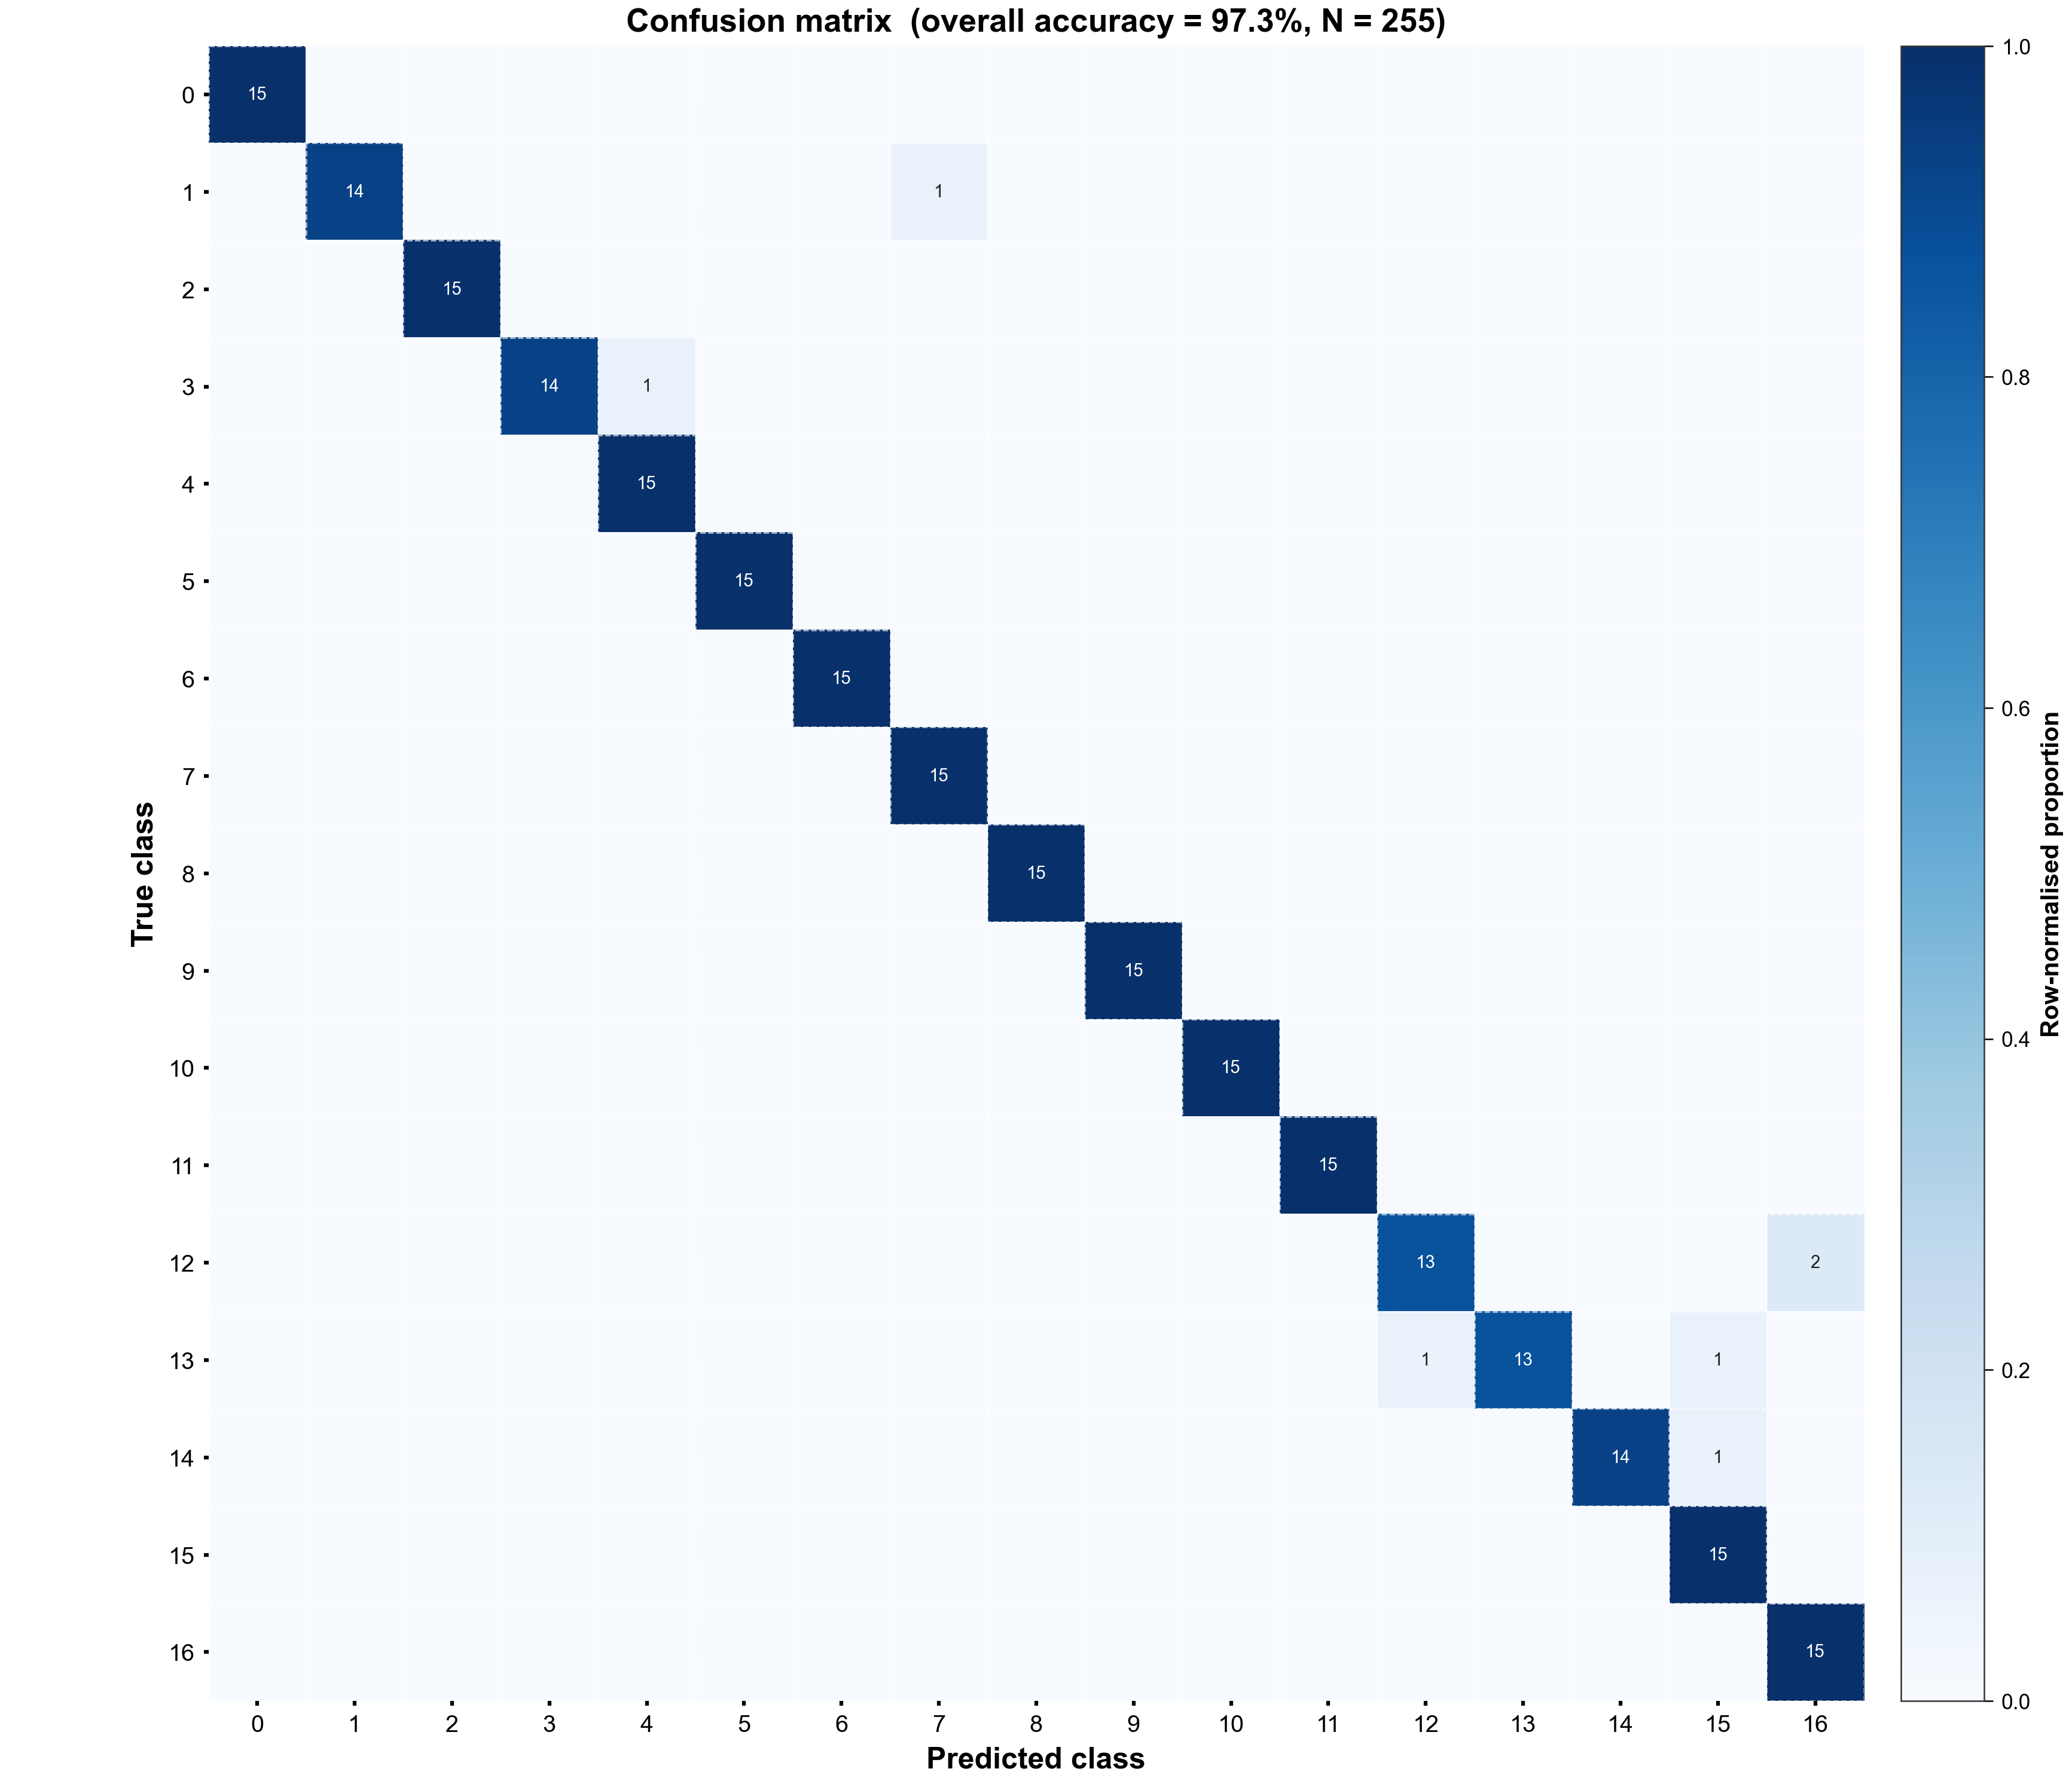
\includegraphics[width=\linewidth]{msca_confusion_matrix.png}
    \caption{Confusion matrix}
  \end{subfigure}\hfill
  \begin{subfigure}{0.48\textwidth}
    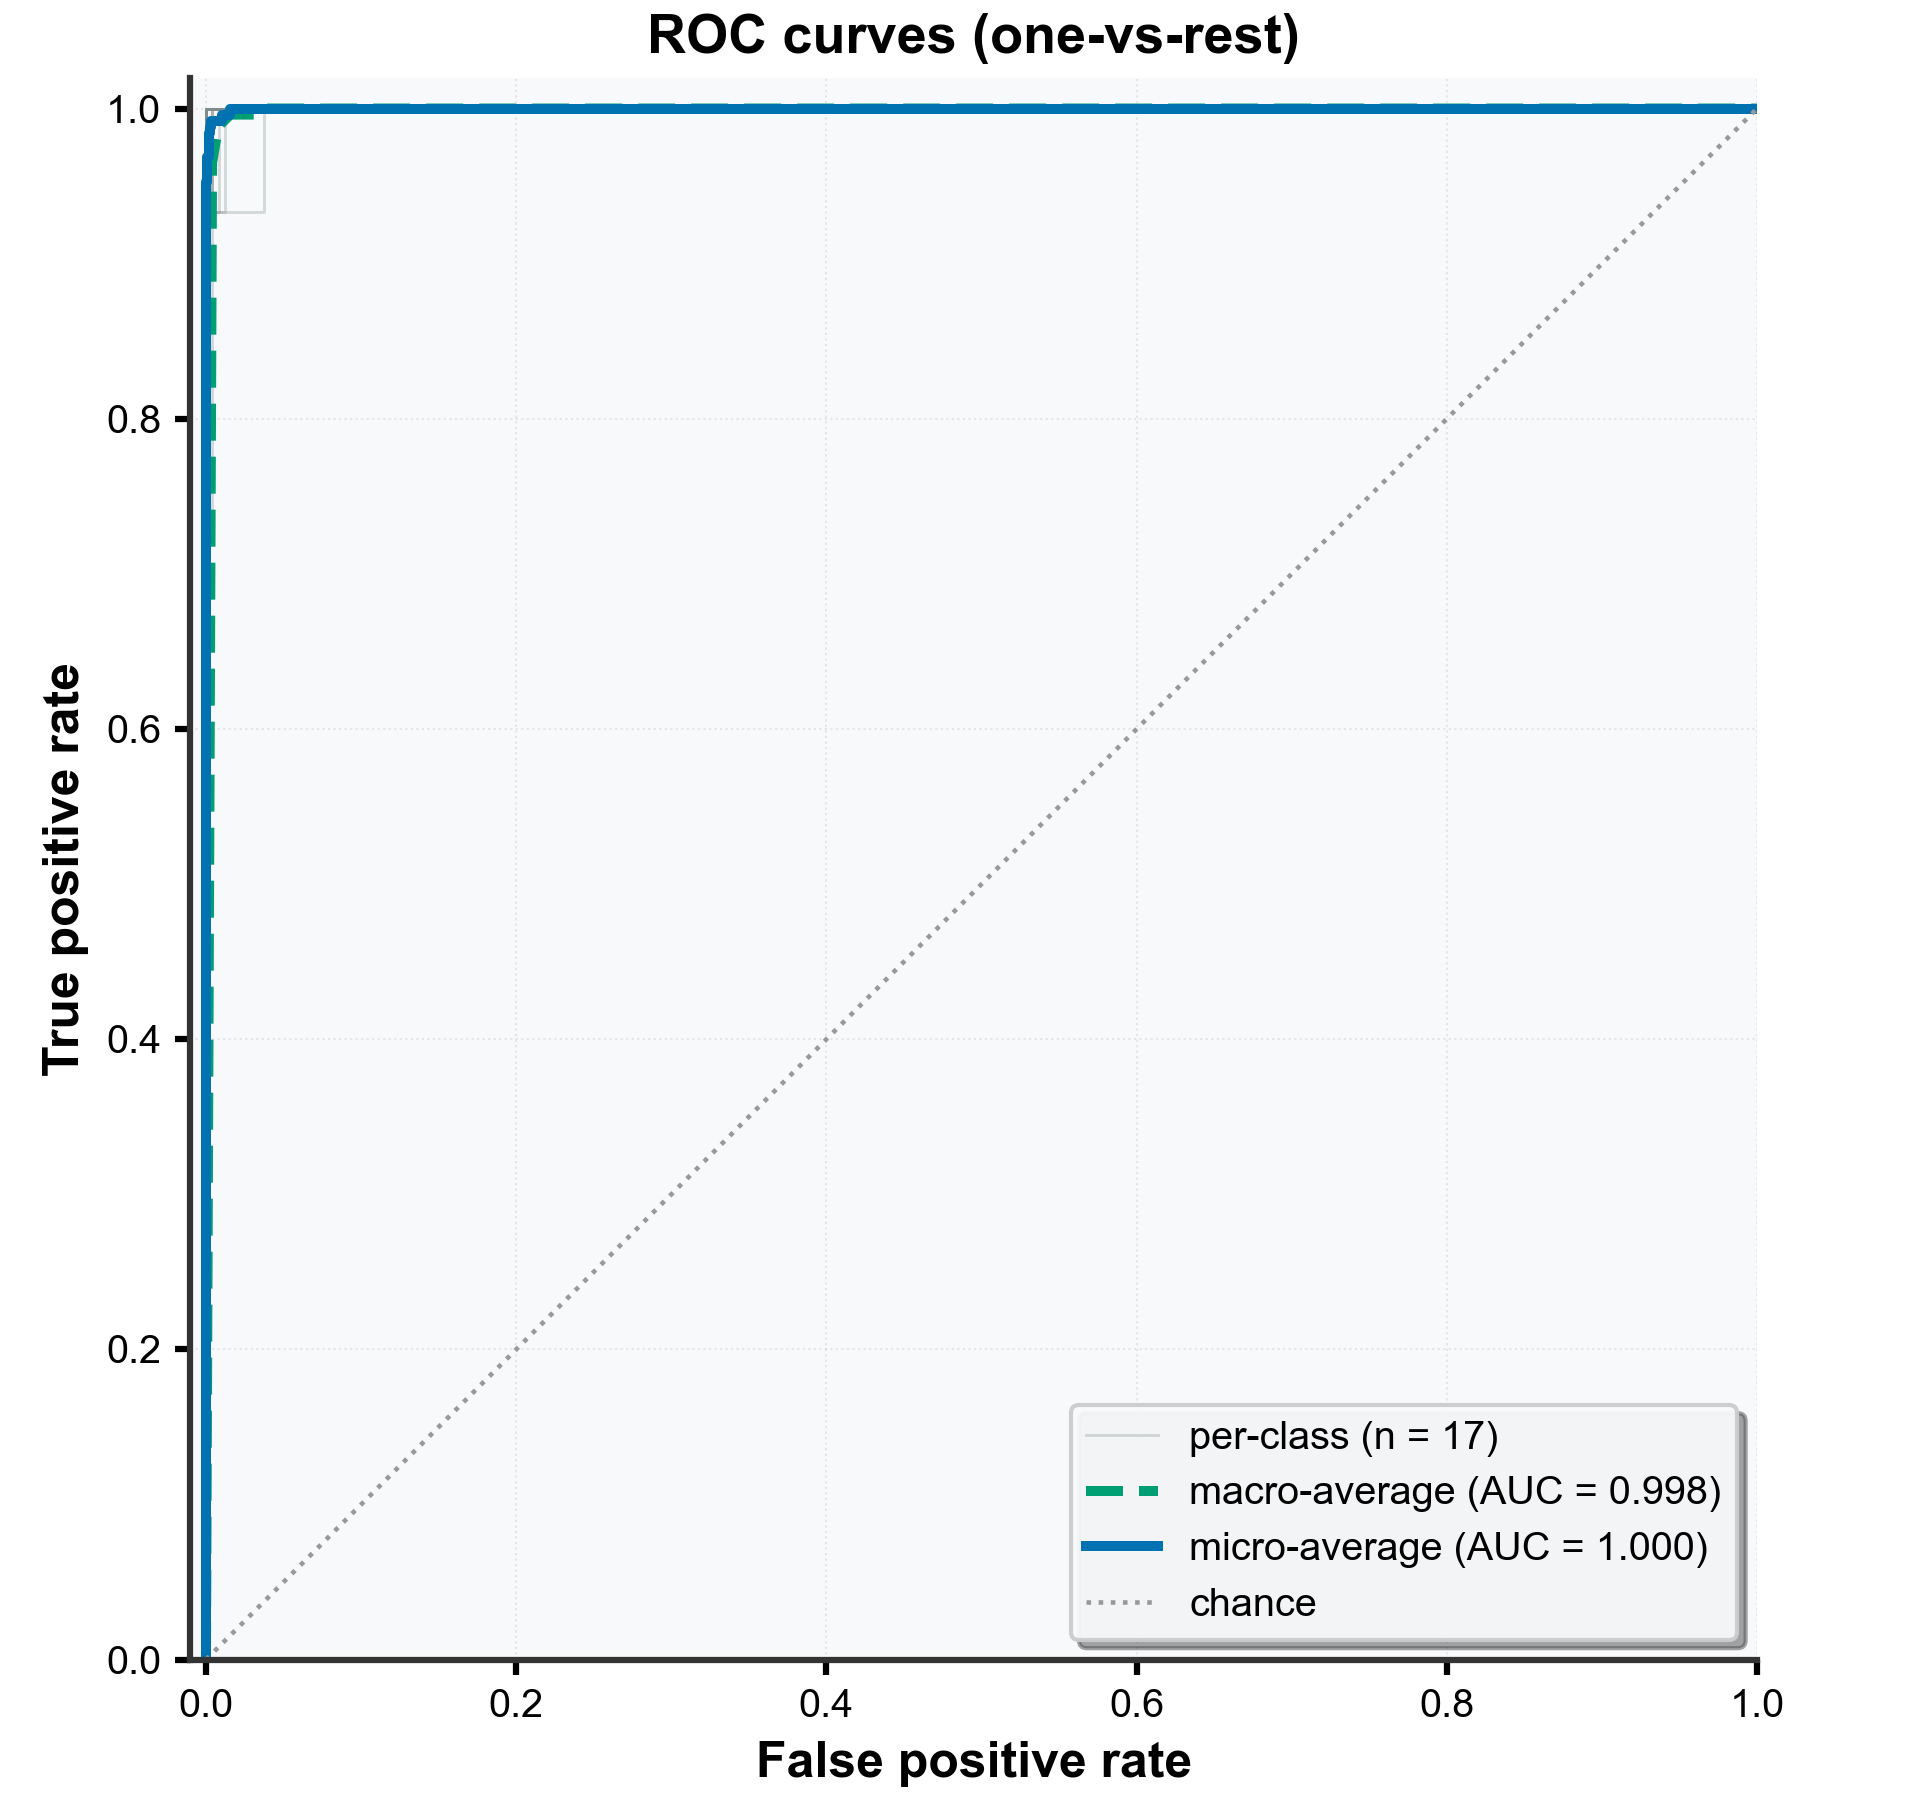
\includegraphics[width=\linewidth]{msca_roc_curve.png}
    \caption{ROC curves (one-vs-rest)}
  \end{subfigure}

  \vspace{0.6em}
  \begin{subfigure}{0.48\textwidth}
    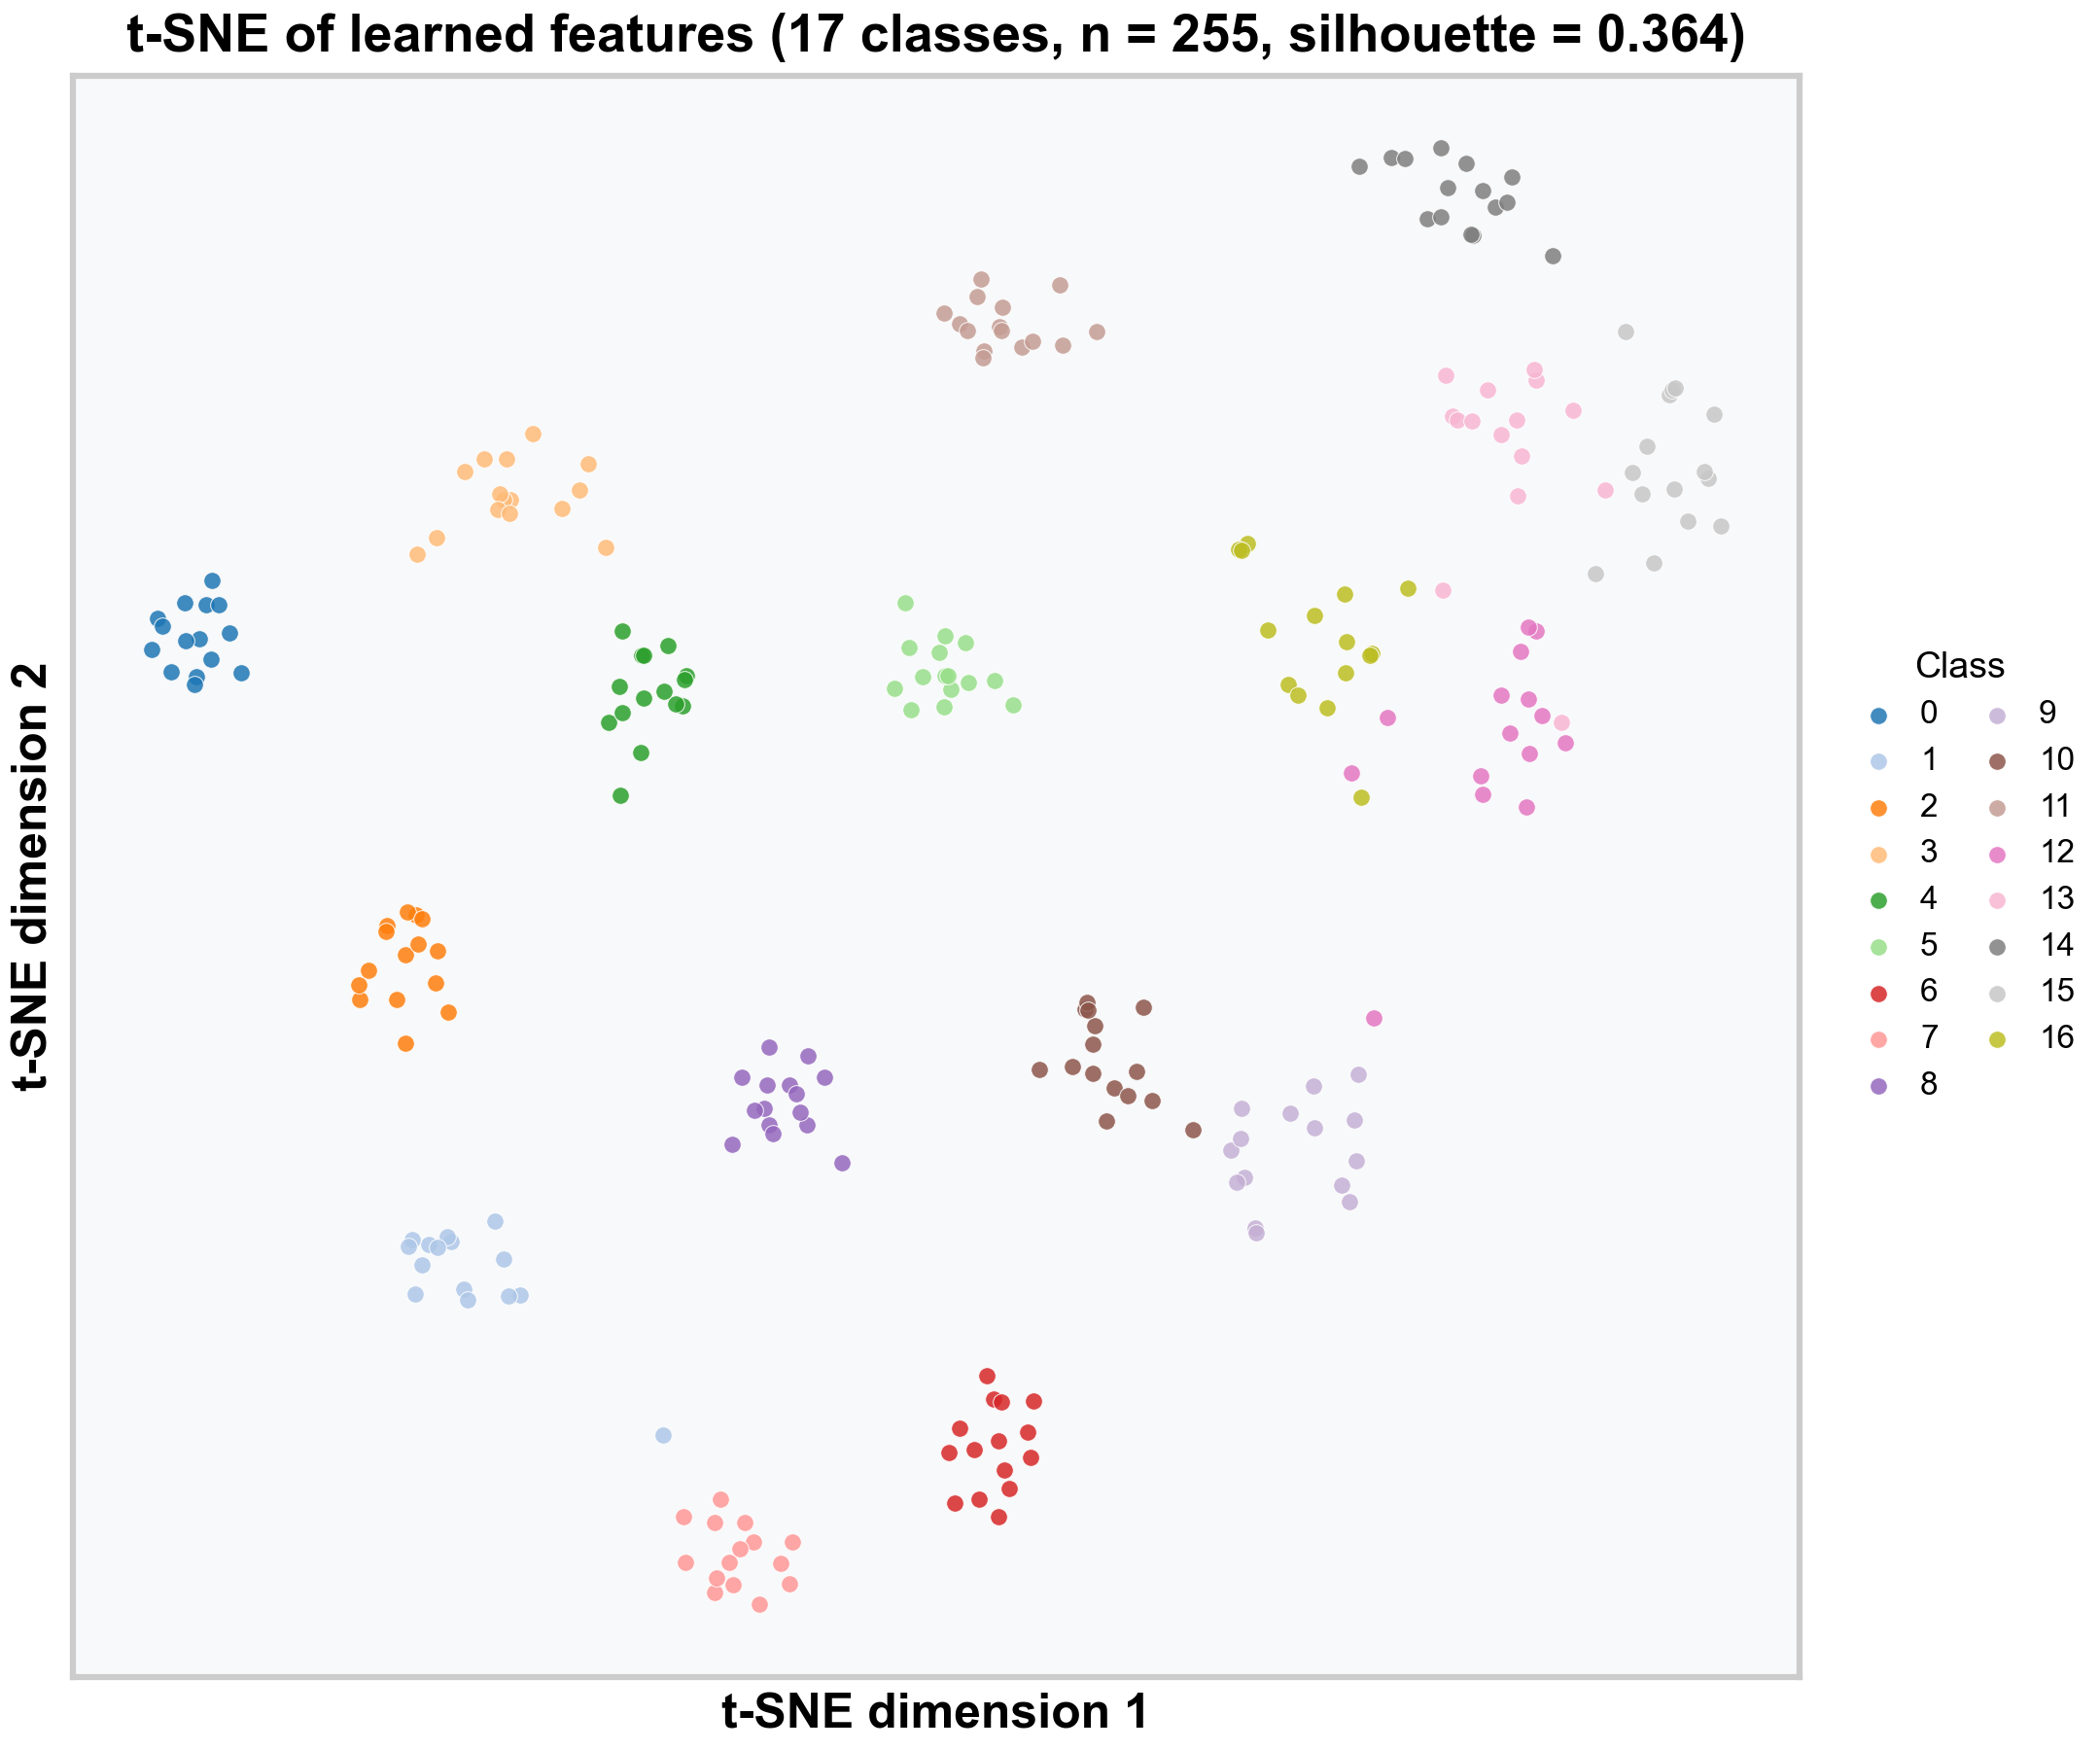
\includegraphics[width=\linewidth]{msca_tsne.png}
    \caption{t-SNE of features}
  \end{subfigure}\hfill
  \begin{subfigure}{0.48\textwidth}
    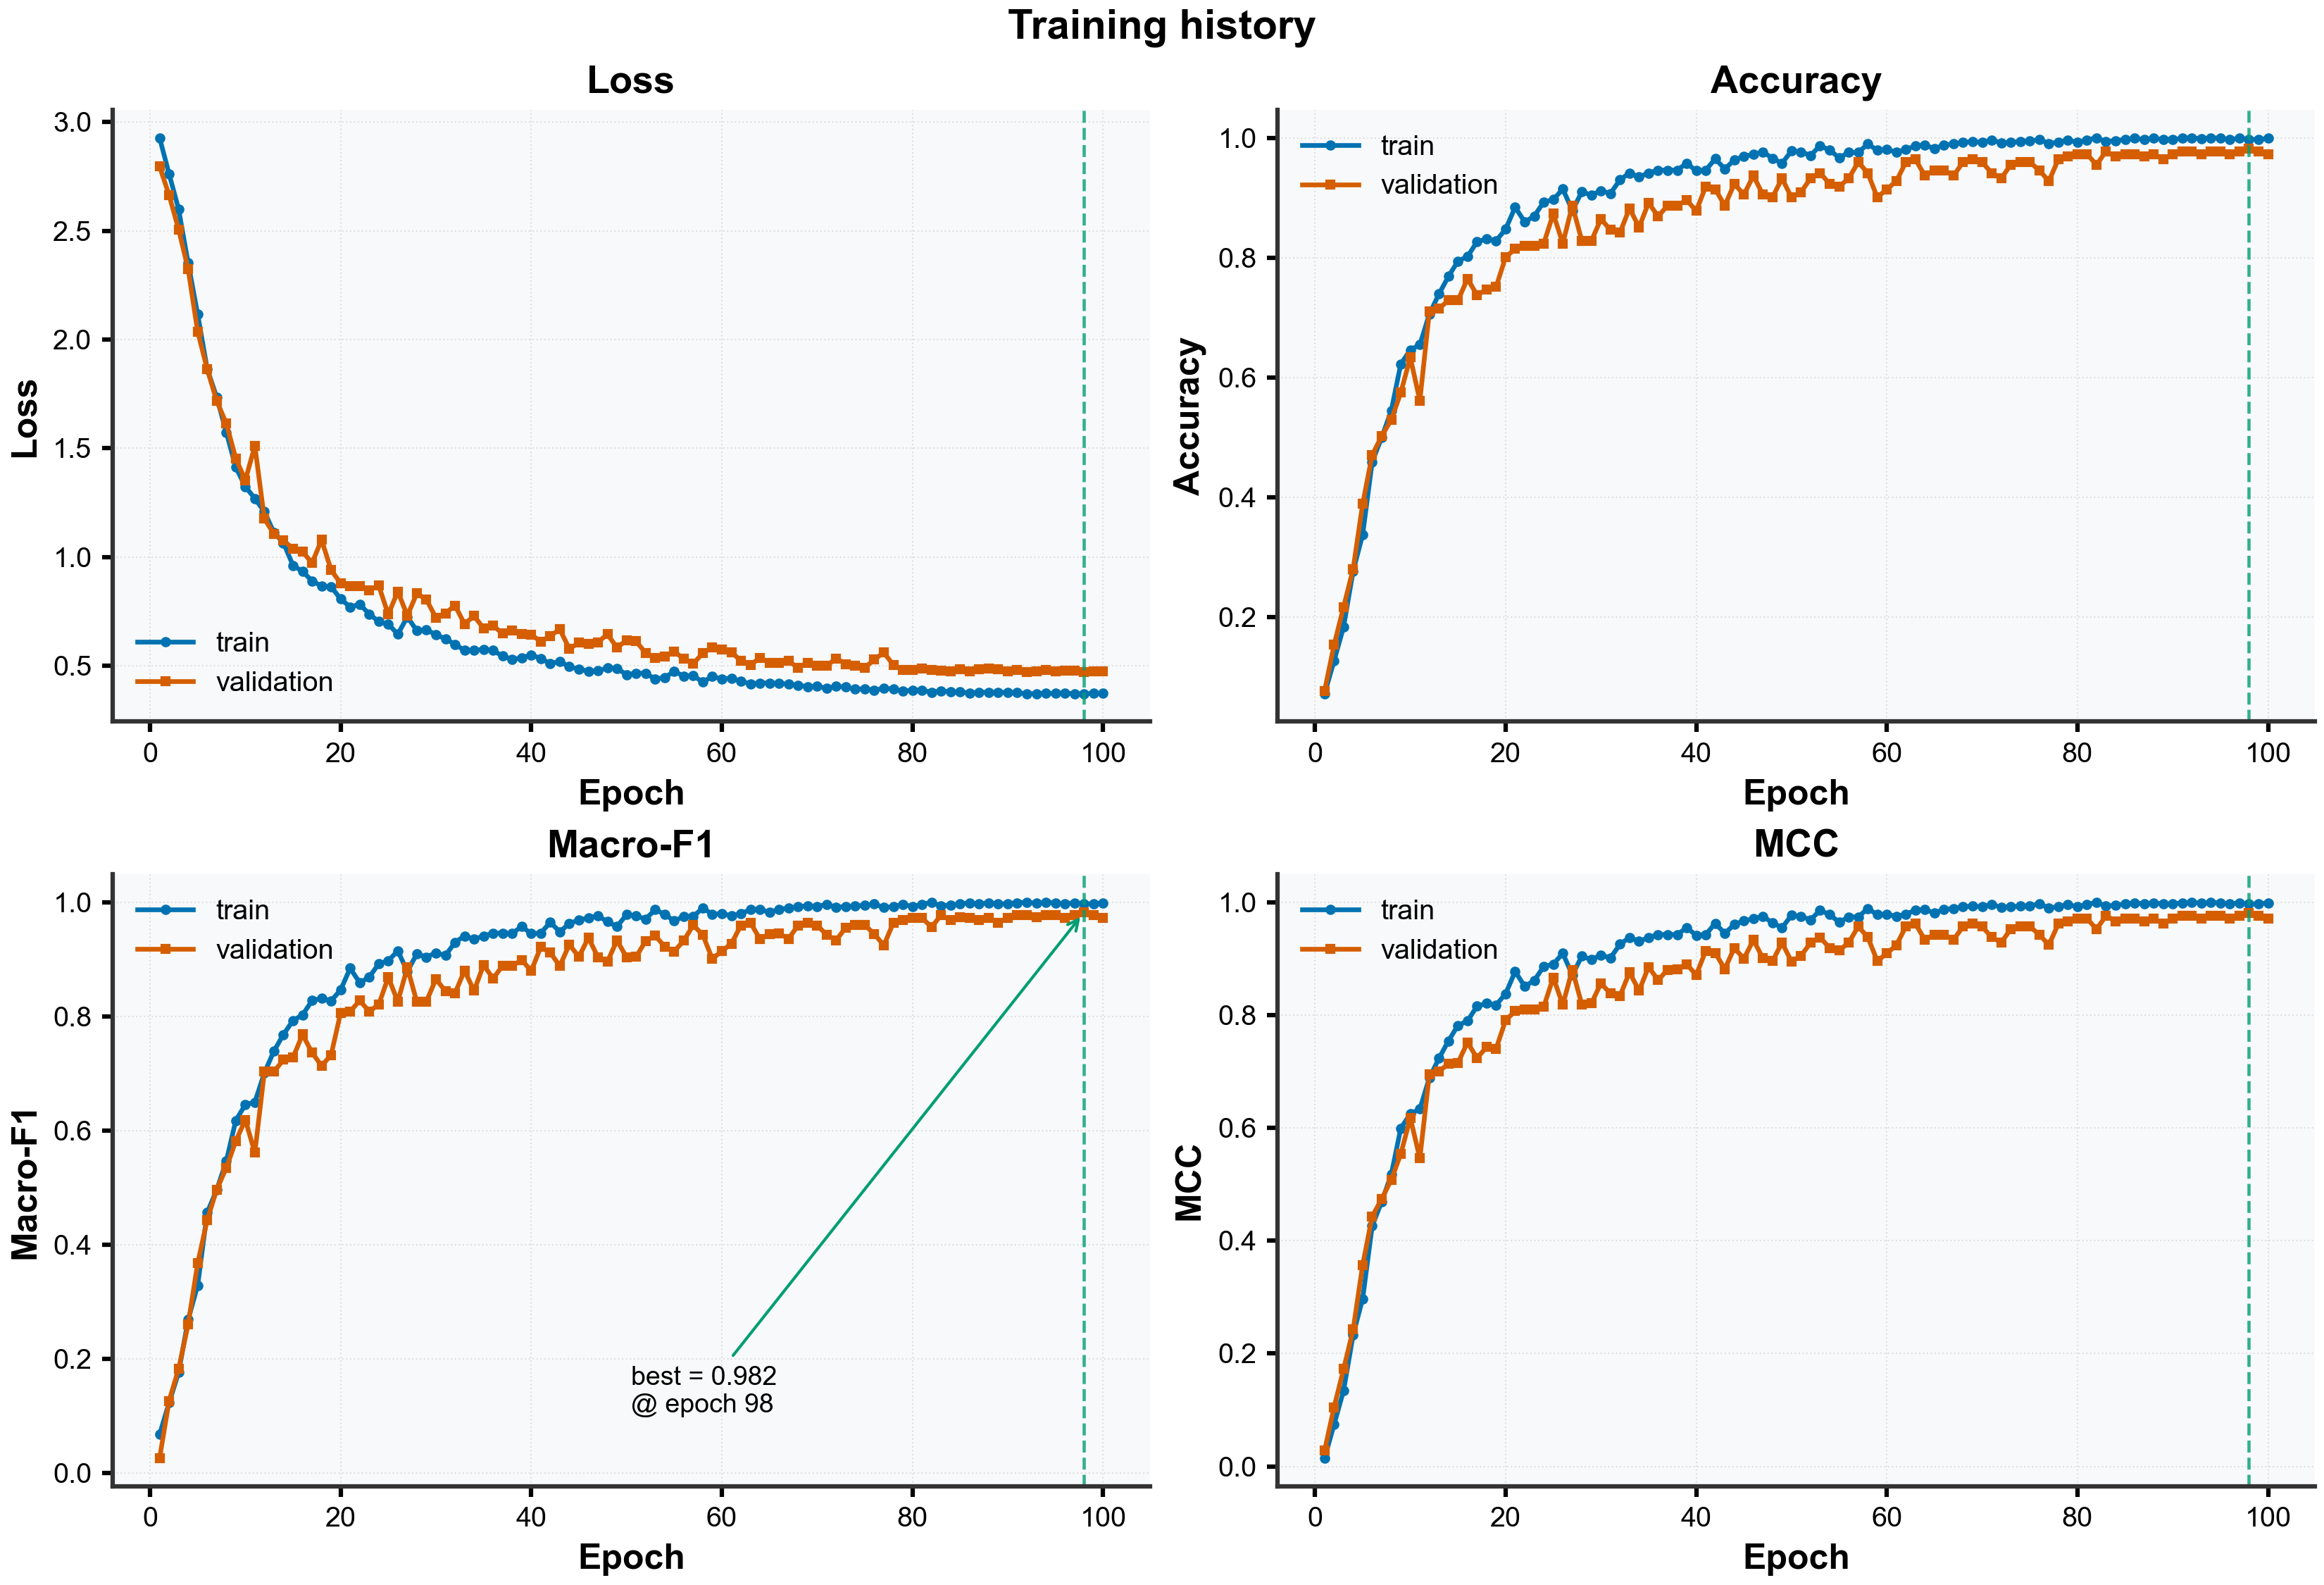
\includegraphics[width=\linewidth]{msca_history.png}
    \caption{Training history}
  \end{subfigure}
  \caption{Diagnostics for MSCA-G on the Z24 test set.}
  \label{fig:diagnostics}
\end{figure}

\section{Discussion}
The results indicate that, for this benchmark, convolutional models dominate:
a well-tuned ResNet-1D is a strong competitor, yet MSCA-G matches and slightly
exceeds it with roughly a quarter of the parameters by combining multi-scale
features, a learned cross-sensor graph, and lightweight attention. The adaptive
graph adds \num{3.5} accuracy points for roughly a thousand extra parameters,
supporting the view that explicitly modelling inter-sensor relations is valuable
for bridge SHM. Recurrent and Transformer baselines lag well behind under the
same budget. The first-order
difference and per-window standardisation remove nuisance amplitude and drift,
which we found more impactful than heavy data augmentation: light jitter together
with single-crop evaluation already yields strong, well-calibrated models whose
training and validation curves behave conventionally. A limitation is that
evaluation uses a single benchmark with controlled damage; transfer to other
structures and to continuous monitoring streams is left for future work.

\section{Conclusion}
We presented MSCA-G, a compact multi-scale convolutional attention network for
vibration-based damage identification. On the Z24 benchmark it outperforms eight
standard time-series baselines under an identical protocol while using a small
parameter budget, and its components are individually justified by an ablation
study. The complete, reproducible
pipeline (data handling, training, evaluation, and publication-quality figures)
is released with this paper.

\section*{Reproducibility}
Code, configurations, and figure-generation scripts are available in the project
repository. All experiments use a fixed seed and deterministic data splits.

\bibliographystyle{unsrt}
\bibliography{references}

\end{document}
